\documentclass[aps,prb,onecolumn,preprint,
	groupedaddress,superscriptaddress,
	amsfonts,amssymb,amsmath,floatfix,
	citeautoscript]{revtex4-1}

\usepackage{graphicx}
\usepackage[centering,hmargin=20mm,tmargin=30mm,bmargin=25mm]{geometry}
\usepackage{multirow}
\usepackage{newtxtext}
\usepackage[cmintegrals]{newtxmath}

%----- References -----
\usepackage{xcolor}
\usepackage{hyperref}
\hypersetup{colorlinks,
	linkcolor={blue!75!black!80!yellow},
	citecolor={blue!75!black!80!yellow},
	urlcolor={blue!75!black!80!yellow}
}

%----- Captions in sans font -----
\makeatletter
\renewcommand\@make@capt@title[2]{%
	\@ifx@empty\float@link{\@firstofone}{\expandafter\href\expandafter{\float@link}}%
	\sffamily{\textbf{#1}}\@caption@fignum@sep#2
}%
\renewcommand\figurename{Fig.}
\makeatother

\thickmuskip=5mu plus 2mu minus 1mu  %binary relations (default, 5mu plus 5mu)
\medmuskip=4mu plus 2mu minus 2mu    %binary operations (default, 4mu plus 2mu minus 4mu)

\frenchspacing %Ensure that revTeX does not do "double spaces" after punctuation

\renewcommand{\Im}{\operatorname{Im}}
\renewcommand{\Re}{\operatorname{Re}}
\newcommand{\sub}[1]{\ensuremath{_{\textrm{#1}}}} %Upright multi-character subscript
\newcommand{\super}[1]{\ensuremath{^{\textrm{#1}}}} %Upright multi-character superscript

\newcommand{\HarvardSEAS}{John A. Paulson School of Engineering and Applied Sciences, Harvard University, Cambridge, MA, USA}
\newcommand{\MITPhy}{Department of Physics, Massachusetts Institute of Technology, Cambridge, MA, USA}

\usepackage[normalem]{ulem}
\newcommand{\Jadd}[1]{\textcolor{blue}{#1}}
\newcommand{\Jrem}[1]{\textcolor{blue}{\sout{#1}}}


%\usepackage[usenames]{color}
%\newcommand{\edited}[1]{{\color{red} #1}}

\begin{document}

\title{Supplementary information: Variational theory of non-relativistic quantum electrodynamics}

\author{Nicholas Rivera}\email{nrivera@seas.harvard.edu}\affiliation{\HarvardSEAS}\affiliation{\MITPhy}
\author{Johannes Flick}\email{flick@seas.harvard.edu}\affiliation{\HarvardSEAS}
\author{Prineha Narang}\email{prineha@seas.harvard.edu}\affiliation{\HarvardSEAS}


\date{\today}


\maketitle
In this Supplement, we derive a self-consistent extension of the equations describing the ground state of a general quantum electrodynamical system with the effect of correlations included. We derive the equations in the case of a multi-electron system in three spatial dimensions interacting quantum electrodynamically with an arbitrary number of photonic modes. The resulting equations are similar in spirit to the equations of quantum electrodynamical density-functional theory~\cite{tokatly2013,ruggenthaler2014} in an optimized-effective potential scheme~\cite{pellegrini2015,flick2017c}, except that the orbitals used in that scheme are Kohn-Sham orbitals, while ours essentially are mean-field orbitals. We then derive the one-dimensional model used in the main text, as well as describe the parameters used in generating the data of Fig. 2 of the main text.

\section{Self-consistent lamb shift correction to the equations for the quantum electrodynamical ground state}

In the derivation of Equations (6) and (7) of the main text, it is notable that the term linear in the vector potential makes no contribution to the expectation value of the Hamiltonian in the ground state. In many quantum electrodynamical problems, this linear term is important. To first order, it leads to spontaneous emission of a single photon. To second order, it leads to Casimir-Polder forces on emitters, which arise from virtual emission and re-absorption of photons. At the same order, the term linear in the vector potential also leads to effective interactions betweeen distinct emitters. Thus, we must capture the effect of this term. Physically, this term mixes the factorizable ground state of Equation (4) of the main text with states that have virtual excitations of the matter, as well as virtual excitations of the electromagnetic field. The resulting state is now non-factorizable and we thus conclude that the term in the Hamiltonian linear in the vector potential leads to \textit{correlations} in the system, and contributes wholly at lowest order to the \textit{correlation energy} of the quantum electrodynamical ground state.

We capture the effect of correlations perturbatively. In other words, we consider the second-order correction $\delta E$ to the ground state energy arising from the term in the Hamiltonian linear in the vector potential. That correction is given by
\begin{equation}
\delta E = \frac{e^2\hbar^2}{8m^2\epsilon_0}\sum\limits_{q=1}^{\infty}\sum_{n=N_{\sigma}+1}^{\infty}\sum\limits_{m=1}^{N_{\sigma}} \frac{\Big| \int d^3x~\mathbf{F}_q^*(\mathbf{x})\cdot\mathbf{j}_{nm}(\mathbf{x})\Big|^2}{\omega_q(\omega_{mn} -\lambda_q)},
\end{equation}
where $\mathbf{j}_{nm} = \psi^*_n\nabla\psi_m - (\nabla\psi^*_n)\psi_m$ are transition current densities, $\omega_{mn} = \omega_m - \omega_n$ are transition frequencies, $N_{\sigma}$ is the number of occupied orbitals, the $\textbf{F}_q$ are the photon mode functions, the $\omega_q$ are the photon mode frequencies, and the $\lambda_q$ are Lagrange multipliers expressing the normalization of each photon mode. We note that the sum over photon modes $q$ is in principle over all modes but can be restricted to either a finite or countably infinite set of photon modes deemed relevant to the system at hand.  In a method without self-consistency, the electron and photon orbitals and eigenvalues are those obtained from Equations (6) and (7) of the main text. This non-self-consistent procedure was applied in Fig. 2 of the main text. In what follows, we add this energy correction $\delta E$ to the expectation value of the energy in the ground state self-consistently, with the orbitals and eigenvalues as variational parameters. As a result, the orbitals and eigenvalues obtained will be different from Equations (6) and (7) of the main text, this difference being small in the case of weak correlations. Strictly speaking, this approach is only justified for weak correlations, but can be applied to systems with strong-correlations as is often done with self-consistent methods. 

\subsection{Physics contained in these equations}

As the equations which result from self-consistence are complicated, it is useful to discuss what physics should contained by introducing $\delta E$ to the Lagrange function to be minimized. From the standpoint of the electrons, the equation for the electron orbitals should differ from Equation (6) of the main text by a potential energy term which corresponds to the spatially dependent Lamb shift  that the electrons feel. This Lamb shift is due to virtual emission and re-absorption of photons. We note in passing that the gradient of the Lamb shift with respect to position gives rise to a force called the Casimir-Polder force.  It is known that this potential depends on all occupied and unoccupied electron orbitals and the photon orbitals, as well as their respective eigenvalues. 

For the photon, the equation will differ from Equation (7) of the main text by the introduction of a term which has the appearance of a source term proportional to a sum over the transition current densities of the electronic system, $\mathbf{j}_{nm}$. These transition currents connect occupied and unoccupied electronic orbitals. The weight of these transition current densities will be proportional to the coupling between the current densities and the photonic modes. In other words, this new term expresses a coupling of the electromagnetic field to fluctuating currents associated with the matter part of the ground state of the QED system. 

\subsection{Equations for the ground state of quantum electrodynamics}

Here, we derive the equations implied by the correction to the energy of Equation (1) and confirm the physical understanding presented in the previous two paragraphs.

The derivative of $\delta E$ with respect to an occupied electron orbital $k$ is given by
\begin{equation}
\frac{\partial\delta E}{\partial \psi_k^*} = \frac{e^2\hbar^2}{8m^2\epsilon_0}\sum\limits_{n=N_{\sigma}+1}^{\infty}\sum\limits_{q=1}^{\infty} \frac{\int d^3y~\mathbf{F}^*_q(\mathbf{y})\cdot\mathbf{j}_{nk}(\mathbf{y})}{\omega_q(\omega_{kn}-\lambda_q)}\int d^3x~\left( \mathbf{F}_q(\mathbf{x})\cdot\nabla\psi_n(\mathbf{x}) + \nabla\cdot(\mathbf{F}_q(\mathbf{x})\psi_n(\mathbf{x}))\right)
\end{equation}
A similar equation arises for the derivative with respect to an unoccupied electron orbital, except that the summation should now be over unoccupied electron orbitals.

The derivative of $\delta E$ with respect to a photonic orbital $q$ is given by
\begin{equation}
\frac{\partial\delta E}{\partial \mathbf{F}_q^*}=\frac{e^2\hbar^2}{8m^2\epsilon_0}\sum\limits_{n=N_{\sigma}+1}^{\infty}\sum\limits_{m=1}^{N_{\sigma}} \frac{\int d^3y~\mathbf{F}_q(\mathbf{y})\cdot \mathbf{j}_{mn}(\mathbf{y})}{\omega_q(\omega_{mn}-\lambda_q)}\mathbf{j}_{nm}(\mathbf{x}).
\end{equation}

The derivative of $\delta E$ with respect to a photonic frequency $\omega_q$ is given by
\begin{equation}
\frac{\partial\delta E}{\partial\omega_q}=-\frac{e^2\hbar^2}{8m^2\epsilon_0}\sum\limits_{n=N_{\sigma}+1}^{\infty}\sum\limits_{m=1}^{N_{\sigma}}\frac{\Big|\int d^3x~\mathbf{F}_q(\mathbf{x})\cdot\mathbf{j}_{mn}(\mathbf{x})\Big|^2}{\omega_q^2(\omega_{mn}-\lambda_q)}
\end{equation}

Using these derivatives, Equation (6) of the main text is generalized to:
\begin{align}
&\left(\frac{\mathbf{p}^2}{2m}+v_{ext}(\mathbf{x}) \right)\psi_i(\mathbf{x}) +  \sum\limits_{j=1}^N \int d^3x' ~ V(\mathbf{x}-\mathbf{x}')\left(\psi^*_j(\mathbf{x}')\psi_j(\mathbf{x}')\psi_i(\mathbf{x}) - \psi_j^*(\mathbf{x}')\psi_j(\mathbf{x})\psi_i(\mathbf{x}')  \right) \nonumber \\ &+ \frac{\hbar e^2}{4m\epsilon_0}\sum_n \frac{1}{\omega_n}|\mathbf{F}_n(\mathbf{x})|^2\psi_i(\mathbf{x}) + \frac{e^2\hbar^2}{8m^2\epsilon_0}\sum\limits_{n=N_{\sigma}+1}^{\infty}\sum\limits_{q=1}^{\infty} \frac{\int d^3y~\mathbf{F}^*_q(\mathbf{y})\cdot\mathbf{j}_{ni}(\mathbf{y})}{\omega_q(\omega_{in}-\lambda_q)}\left( \mathbf{F}_q(\mathbf{x})\cdot\nabla\psi_n(\mathbf{x}) + \nabla\cdot(\mathbf{F}_q(\mathbf{x})\psi_n(\mathbf{x}))\right)  \nonumber \\ &= E_i\psi_i(\mathbf{x}).
\end{align}

Setting the derivative with respect to photonic modes zero gives the equation:
\begin{equation}
\frac{\hbar}{4}\left(\omega_q\mathbf{F}_q(\mathbf{x}) + \frac{c^2}{\omega_q}\nabla\times\nabla\times\mathbf{F}_q(\mathbf{x})\right) + \frac{\hbar\sum\limits_{m=1}^{N_{\sigma}}|\psi_m(\mathbf{x})|^2}{4m\epsilon_0\omega_q}+\frac{e^2\hbar^2}{8m^2\epsilon_0}\sum\limits_{n=N_{\sigma}+1}^{\infty}\sum\limits_{m=1}^{N_{\sigma}}\frac{\int d^3y ~\mathbf{F}_q(\mathbf{y})\cdot\mathbf{j}_{mn}(\mathbf{y})}{\omega_q(\omega_{mn}-\lambda_q)}\mathbf{j}_{nm}(\mathbf{x}) = \frac{\hbar\lambda_q}{2}\mathbf{F}_q(\mathbf{x})
\end{equation}

And setting the derivative with respect to the photonic frequencies to zero gives the equation:
\begin{align}
&\frac{\hbar}{4}\left(\int d^3x ~|\mathbf{F}_q(\mathbf{x})|^2 - \frac{c^2}{\omega_q^2}\mathbf{F}^*_q(\mathbf{x})\cdot\nabla\times\nabla\times\mathbf{F}_q(\mathbf{x}) \right) - \frac{e^2\hbar}{4m\epsilon_0\omega_q^2}\int d^3x~\sum\limits_{m=1}^{N_{\sigma}} |\psi_m(\mathbf{x})|^2 \nonumber \\ &-\frac{e^2\hbar^2}{8m^2\epsilon_0}\sum\limits_{n=N_{\sigma}+1}^{\infty}\sum\limits_{m=1}^{N_{\sigma}}\frac{\Big|\int d^3x~\mathbf{F}_q(\mathbf{x})\cdot\mathbf{j}_{mn}(\mathbf{x})\Big|^2}{\omega_q^2(\omega_{mn}-\lambda_q)}=  0 
\end{align}
Performing the operation $\frac{1}{\omega_q}\int d^3x \mathbf{F}_q^*(\mathbf{x})  \cdot$ on Equation (6), and adding the result to Equation (7), gives the result $\lambda_q = \omega_q$, just as before $\delta E$ was introduced. Using this key simplification, along with the definition of the spatially-dependent plasma frequency as $\omega_p^2(\mathbf{x}) = \frac{e^2}{m\epsilon_0}\sum\limits_{m=1}^{N_{\sigma}}|\psi_m(\mathbf{x})|^2$, we have that Equation (7) of the main text is generalized to:
\begin{equation}
\left( \nabla\times\nabla\times - \left(1-\frac{\omega_p^2(\mathbf{x})}{\omega_q^2} \right)\right)\mathbf{F}_q(\mathbf{x}) = -\frac{e^2\hbar}{2m^2\epsilon_0c^2}\sum\limits_{n=N_{\sigma}+1}^{\infty}\sum\limits_{m=1}^{N_{\sigma}} \frac{\int d^3y~\mathbf{F}_q(\mathbf{y})\cdot\mathbf{j}_{mn}(\mathbf{y})}{\omega_{mn}-\omega_{q}}\mathbf{j}_{nm}(\mathbf{x}).
\end{equation}
\textit{Equations (5) and (8) represent main results of this work and provide a general starting point for first-principles analysis of ground states of QED systems in the non-perturbative regime.}

\section{Derivation of results for one-dimensional cavity model in the main text}

In this section, we provide some additional details on the one-dimensional cavity QED model considered in the main text. Given the Hamiltonian of Equation (9) in the main text describing the coupling of an emitter to a one-dimensional cavity, with the matter being described by the site model of Equations (10) and (11) of the main text, the expectation value of the Hamiltonian according to the ansatz of Equation (4) in the main text is given by
\begin{equation}
\langle \Psi | H | \Psi \rangle = \langle \tilde{g} |H_{\text{matter}} | \tilde{g}\rangle + \frac{\hbar}{4}\int dz ~\sum\limits_{n=1}^{\infty}\left(\omega_n|F_n|^2 - \frac{c^2}{\omega_n}F_n^*\partial_z^2F_n\right) + \frac{\hbar q^2}{4m\epsilon_0\omega_n}\sum\limits_{n=1}^{\infty} \int dz~\delta(z-d)|F_n|^2
\end{equation}
In this equation, $|\tilde{g}\rangle$ is the ground state of the effective matter part of the Hamiltonian, and $H_{\mathrm{matter}}$ is the Hamiltonian of Equation (10) of the main text.  We impose constraints of matter normalization and photon mode normalization by defining a Lagrange function 
\begin{equation}\label{eq:lagrange}
\mathcal{L}(|\tilde{g}\rangle, \langle \tilde{g}|,\epsilon, \{F_n, F_n^*, \omega_n, \lambda_n\}) \equiv \langle \Psi | H | \Psi \rangle - \epsilon(\langle \tilde{g}|\tilde{g}\rangle-1)-\sum\limits_{n=1}^{\infty}\frac{\hbar\lambda_n}{2}\left( \int dz~|F_n|^2-1\right).
\end{equation} 
To find the ground state, we minimize the Lagrange function with respect to the matter orbital $|\tilde{g}\rangle$ and with respect to the mode functions $F_n$. The minimization with respect to the matter leads to the trivial equation $H_{\text{matter}} |\tilde{g}\rangle = \epsilon|\tilde{g}\rangle$ which leaves the effective matter ground state as simply the ground state of $H_{\text{matter}}$. On the other hand, the minimization with respect to the photon mode functions leads to  the equation
\begin{equation}\label{eq:maxwell}
\left(\partial_z^2-\frac{\omega^2_n}{c^2}+2\frac{\omega_n\lambda_n}{c^2}-\frac{q^2 }{m\epsilon_0 c^2}\delta(z-d)\right)F_n  = 0.
\end{equation}
We may constrain the $\lambda_n$ by differentiating the Lagrange function with respect to the $\omega_n$. The equation which follows is:
\begin{equation}\label{eq:other_maxwell}
\int dz ~\left(|F_n|^2 + \frac{c^2}{\omega^2_n}F_n^*\partial_z^2F_n\right) - \frac{ q^2}{m\epsilon_0\omega^2_n} \int dz~\delta(z-d)|F_n|^2 = 0
\end{equation}
Performing $\frac{\omega_n^2}{c^2}\int dz~F_n^*$ on both sides of Equation (11), and adding this equation to Equation (12), one immediately finds that $\lambda_n = \omega_n$ and that
\begin{equation}\label{eq:final_maxwell}
\left(\partial_z^2+\frac{\omega^2_n}{c^2}-\frac{q^2 }{m\epsilon_0 c^2}\delta(z-d)\right)F_n  = 0.
\end{equation}

This is an ordinary second-order differential equation with the conditions that $F_n$ is continuous at $d$ and that its derivative is discontinuous according to 
\begin{equation}\label{eq:boundary_condition}
\partial_zF_n\Big|_{z=d^+}-\partial_zF_n\Big|_{z=d^-} = \frac{q^2}{m\epsilon_0 c^2}F_n(d),
\end{equation}
in addition to the usual condition of the modes vanishing at the cavity walls $z=0$ and $z=L$. It can be shown that the solution to Equation (13) satisfying such boundary conditions is:
\begin{align}\label{eq:field_mode}
&\theta (z-d) \left(\frac{\sin\left(\frac{\omega_nL}{c}\right)\sin\left(\frac{\omega_nd}{c}\right)\cos\left(\frac{\omega_nz}{c}\right)}{\sin\left(\frac{\omega_n(L-d)}{c}\right)}-\right) \nonumber \\ 
-&\theta (z-d) \left(\frac{\cos\left(\frac{\omega_nL}{c}\right)\sin\left(\frac{\omega_nd}{c}\right)\sin\left(\frac{\omega_nz}{c}\right)}{\sin\left(\frac{\omega_n(L-d)}{c}\right)}\right) \nonumber \\ 
+&\theta (d-z) \sin\left(\frac{\omega_n z}{c} \right)
\end{align}
provided that the auxiliary condition
\begin{equation}\label{eq:mode_transcendental}
\cot\left(\frac{\omega_n}{c}d \right)+\cot\left(\frac{\omega_n}{c}(L-d) \right) = -\frac{q^2}{m\epsilon_0\omega_nc}
\end{equation}
is met. To ensure that the modes are normalized according to the constraint, we have that the solutions of Equation (15) must be multiplied by a normalization factor $N_n$ given by
\begin{equation}\label{eq:mode_normalization}
N_n = 2\sqrt{\frac{1}{\frac{c}{\omega_n}\left(\frac{\omega_nL}{c}-\sin\left(\frac{\omega_nL}{c}\right) \right)\left(1+\frac{\sin^2\left(\frac{\omega_nd}{c}\right)}{\sin^2\left(\frac{\omega_n(L-d)}{c}\right)} \right)}}.
\end{equation}
The condition of Equation \ref{eq:mode_transcendental} determines the resonance frequencies of the photon quasiparticle modes. 

\subsubsection{Perturbation theory for the one-dimensional cavity model}

\textcolor{blue}{As discussed in the main text, the variational energies, as well as the energies from numerical diagonalization, are compared against the energies calculated from perturbation theory. We provide additional details on the perturbative calculations here. What we calculate is the energy shift of a state $|a,0\rangle$, where $a$ is any matter state, and $0$ denotes the photonic vacuum, according to the perturbation Hamiltonian $\frac{q}{m}Ap + \frac{q^2}{2m}A^2$, where $p$ is the momentum operator for the matter defined in the main text, and $A$ is the vector potential operator of the one-dimensional cavity in the absence of the matter. In particular, $A(z) = \sum_n\sqrt{\frac{\hbar}{\epsilon_0\omega_n L}}\sin\left(\frac{n\pi z}{L} \right) \left(a_n+a^{\dagger}_n\right)$, with $L$ the length of the cavity and $\omega_n = \frac{n\pi c}{L}$. Upon inspection, it is clear the the $A^2$ term leads to an energy shift at first-order in perturbation theory, while the $A\dot p$ term leads to an energy shift at second-order in perturbation theory. A straightforward application of perturbation theory leads to the following first-order energy shift from the $A^2$ term:
\begin{equation}
\delta E_a = \frac{q^2}{2m}\sum\limits_{n=1}^{N_p} \frac{\hbar}{\epsilon_0\omega_n L}\sin^2\left(\frac{n\pi z}{L}\right),
\end{equation}
where $z$ is the location of the matter in the cavity, and $N_p$ is the maximum photon number retained. Note that this value is dependent on the maximum photon number (although somewhat weakly) retained due to the logarithmically diverging nature of the sum, and so to compare variational, numerical, and perturbative calculations, the same number of modes are retained in each. A similarly straightforward application of perturbation theory leads to the energy shift coming from the $A\dot p$ term being given by:
\begin{equation}
\delta E_a = \frac{q^2}{m^2}\sum\limits_{b\neq a}\sum\limits_{n=1}^{N_p} \frac{\hbar}{\epsilon_0\omega_n L} \frac{|p_{ba}|^2\sin^2\left(\frac{n\pi z}{L} \right)}{\hbar(\omega_a - \omega_b - \omega_n)},
\end{equation}
where $b$ denotes a matter state different from $a$, and $p_{ba} = \langle b|p|a\rangle$.}

\textcolor{blue}{In the main text, we also considered expectation values such as $\langle A \cdot p \rangle$ in the ground state within perturbation theory. Calculating the shift of the ground-state wavefunction at first-order in perturbation theory, we immediately find that
\begin{equation}
\langle Ap \rangle = \frac{2q}{m} \text{Re } \sum\limits_{b\neq a}\sum\limits_{n=1}^{N_p} \frac{1}{2\epsilon_0L}\frac{|p_{ba}|^2\sin^2\left(\frac{n\pi z}{L}\right)}{\omega_n(\omega_a-\omega_b-\omega_n)}.
\end{equation}}

\textcolor{blue}{It is also of interest to consider "field-only" observables such as the number of (virtual) photons in the ground state. Calculating the wavefunction of the ground state at first-order in perturbation theory, and calculating the probability of a photon being in the ground state, one finds that 
\begin{equation}
\langle N \rangle =\sum\limits_{n=1}^{N_p} \langle a^{\dagger}_{n,\text{bare}}a_{n,\text{bare}} \rangle = \frac{q^2}{m^2} \sum\limits_{b\neq a}\sum\limits_{n=1}^{N_p} \frac{1}{2\hbar\epsilon_0L}\frac{|p_{ba}|^2\sin^2\left(\frac{n\pi z}{L}\right)}{\omega_n(\omega_a-\omega_b-\omega_n)^2},
\end{equation}
where the "b" or "bare" subscript in the creation and annihilation operators denotes that these are creation and annihilation operators for photon modes in the cavity in the absence of interactions (e.g., the sine modes for the 1D cavity considered here). In Fig. S1, we compare the expectation value of the number of "bare" photons calculated  perturbatively, and with exact diagonalization with the variationally calculated number of "interacting" photons, $\sum\limits_{n=1}^{N_p} \langle a^{\dagger}_{n,\text{int}}a_{n,\text{int}} \rangle$ (e.g., the modes shown in Fig. 2b of the main text). The number of photons in the bare basis differs substantially from the number of photons in the interacting basis.}

\textcolor{blue}{This behavior does not reflect any inconsistency with the variational method, but is instead a feature which is to be expected. In particular, the physics of the ansatz of Eq. 4 of the main text is that a complicated ground state which has many virtual photons (see numerical diagonalization result) in it should be physically equivalent to a ground state with nearly no virtual photons (see variational result), but with different modes and frequencies. In other words, the reason the number of virtual photons differs is simply because they are being counted in the basis of "interacting modes" shown in Fig. 2b of the main text.   That said, our variational theory does not give a prescription to translate the interacting mode operators to the bare mode operators.}

\begin{figure}[t]
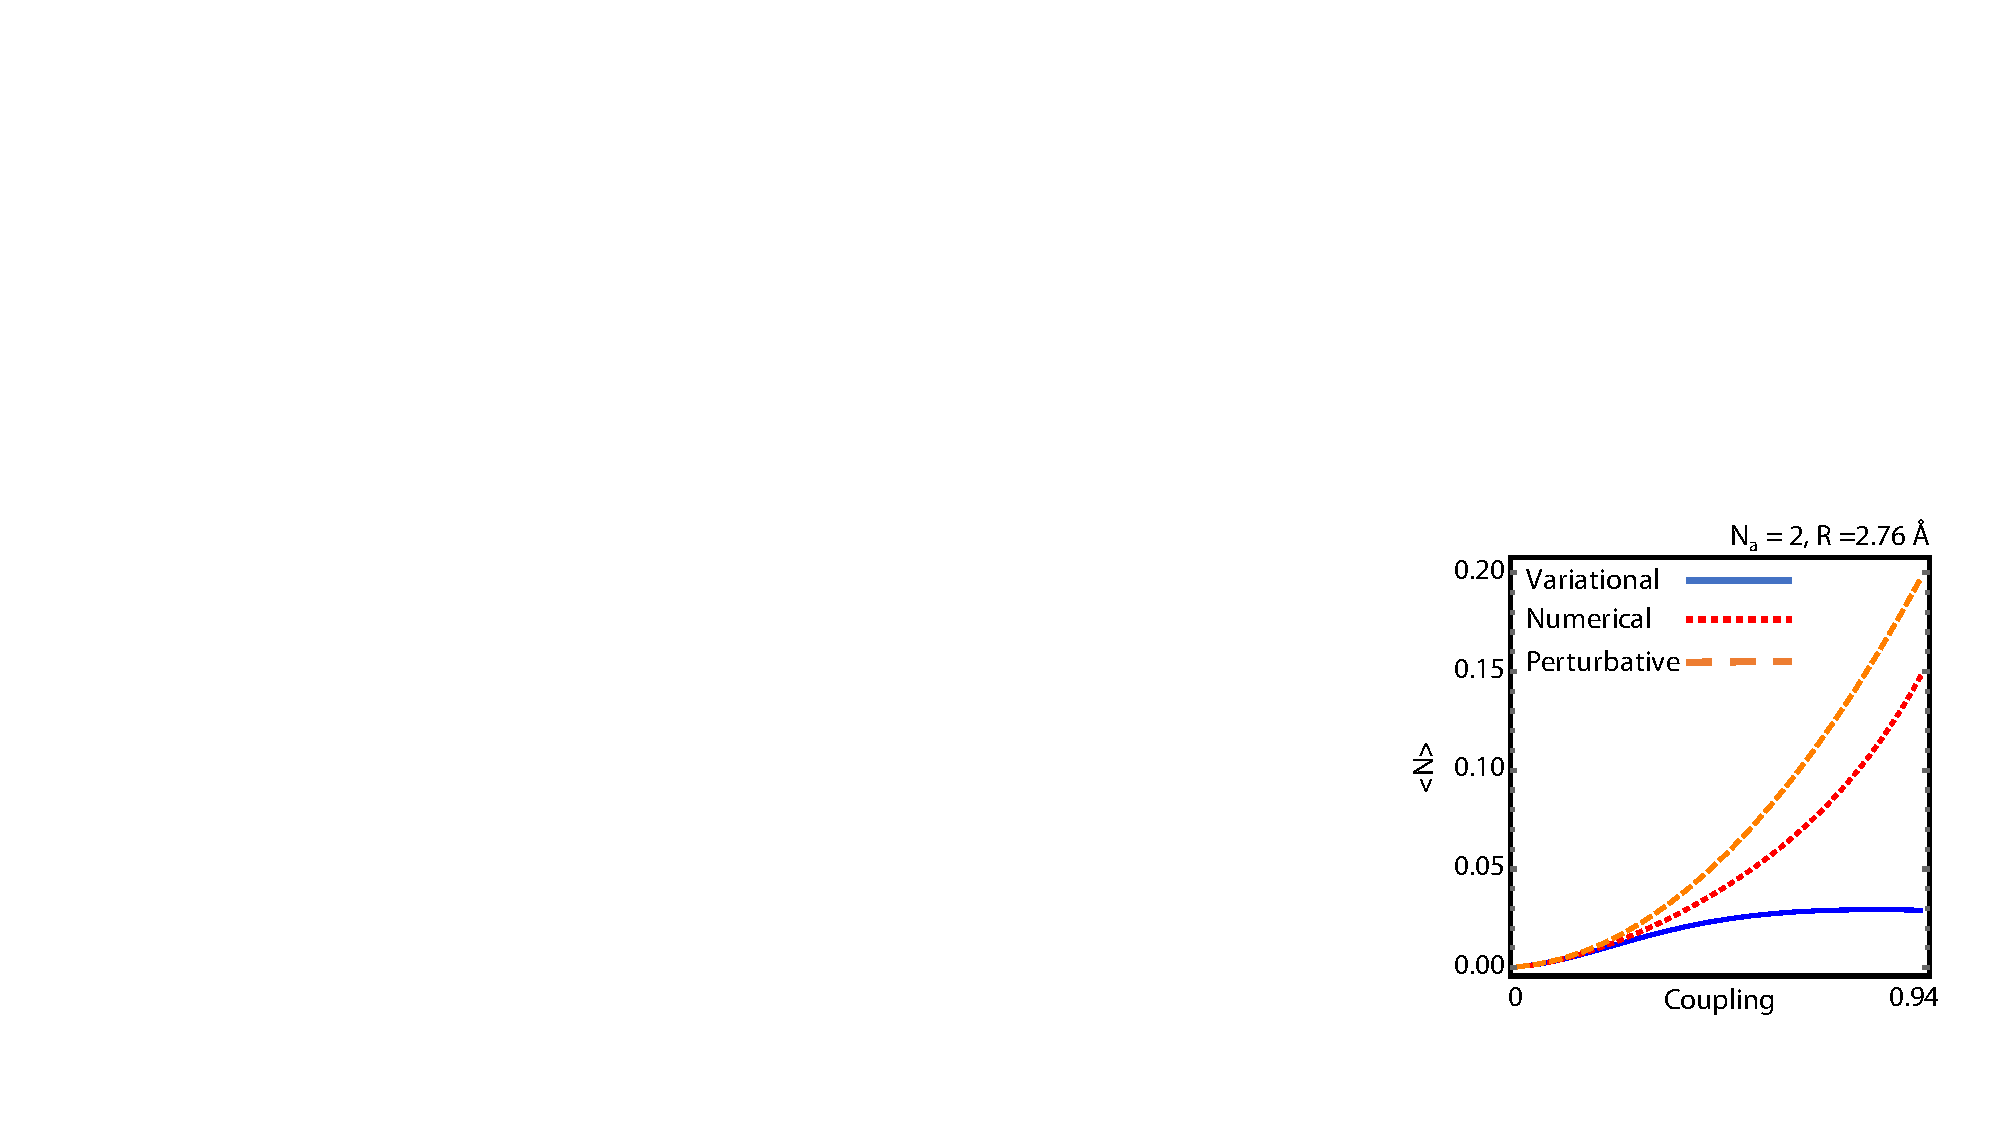
\includegraphics[width=6cm]{FigureS1.pdf}
\caption{\textcolor{blue}{\textbf{Number of virtual photons (bare and interacting) in the ground state calculated variationally, numerically, and through perturbation theory.} Parameters are the same as in Fig. 2 (top panel) of the main text.}}
\label{fig:ansatz}
\end{figure}

\textcolor{blue}{We note that in all cases, when calculating these quantities in the variational theory, these expressions are still relevant, with the replacement of the bare photon frequencies and mode functions replaced by the ones that result from Eq. 7 of the main text.}

\subsection{Model parameters for Figure 2 and details of numerical diagonalization}

Here, we note the parameters used in Fig. 2, as well as some details regarding the numerical diagonalization used to assess the validity of the variational approach advanced in the main text.

\begin{enumerate}
\item{The hopping matrix elements $t$ were taken to be 0.25 eV for the two-, three-, and four-level systems. Meanwhile, the on-site energies were taken to be equal on all sites in the two-, three-, and four-level systems.}
\item{The cavity length was taken to be 1 micron.}
\item{The area of the cavity in the transverse direction was taken to be 100 nm$^2$.}
\item{The maximum number of cavity modes retained in the calculations was 100. Our results were converged with respect to the number of cavity modes.}
\item{In the numerical diagonalization results (red lines of Fig. 2 of the main text), the Fock space was truncated such that the number of photons retained was no more than four. For the largest couplings plotted in Fig. 2, this was sufficient. But for higher couplings, more photons in the numerical diagonalization are needed. For four photons and 100 cavity modes coupled to a four-level system, the dimension of the Hilbert space is  $4\times \left( 1 + 100 + 5050 + 171,700 + 4,421,275 \right) = 18,392,504$. The four terms in the parentheses correspond to the dimension of the properly symmetrized zero-, one-, two-, three-, and four-photon Hilbert spaces respectively. Also see Ref.~\cite{flick2017} for more details on the exact numerical diagonalization methods for light-matter coupled problems.}
\item{The largest couplings plotted in Fig. 2 correspond to either a single emitter with a charge of $200e$, or an ensemble of emitters (as is the case in many ultra-strong coupling experiments) in which there are 40,000 emitters in the cavity. The largest couplings correspond to rather extreme coupling parameters and are shown mostly to demonstrate that our ansatz is quite accurate even in regimes of extremely high coupling.}
\end{enumerate}

\textcolor{blue}{Regarding the numerical diagonalization, we numerically implement the Hamiltonian of Eq. (9) of the main text by building the matter operators ($H_0$ and $p$ as defined in the main text) in the basis of states corresponding to the tensor product of any matter state, and any photon state having four photons or less . Details regarding the ordering convention for the properly symmetrized multi-photon states are provided in Ref.~ \cite{flick2017} for example. Photon operators ($a$, $a^{\dagger}$) are constructed in this basis, and used to construct field operators such as $A$ in the basis of bare cavity modes (the usual sine modes). In particular, $A(z) = \sum_n\sqrt{\frac{\hbar}{\epsilon_0\omega_n L}}\sin\left(\frac{n\pi z}{L} \right) \left(a_n+a^{\dagger}_n\right)$, with $L$ the length of the cavity and $\omega_n = \frac{n\pi c}{L}$. Diagonalization is performed using standard sparse eigendecomposition routines (such as those implemented in MATLAB).}

\bibliographystyle{apsrev4-1}
\bibliography{references}

\end{document}
